\section{ЗАДАНИЕ}

Составить программу, т.е. модель предметной области – базу знаний, объединив в ней информацию – знания:

\begin{itemize}
    \item <<Телефонный справочник>>: Фамилия, №тел, Адрес – структура (Город, Улица, №дома, №кв),
    \item <<Автомобили>>: Фамилия\_владельца, Марка, Цвет, Стоимость, и др.,
    \item <<Вкладчики банков>>: Фамилия, Банк, счет, сумма, др.
\end{itemize}

Владелец может иметь несколько телефонов, автомобилей, вкладов (Факты).

Используя правила, обеспечить возможность поиска:

\begin{enumerate}
    \item По № телефона найти: Фамилию, Марку автомобиля, Стоимость автомобиля (может быть несколько),
    \item Используя сформированное в пункте а) правило, по № телефона найти: только Марку автомобиля (автомобилей может быть несколько),
    \item Используя простой, не составной вопрос: по Фамилии (уникальна в городе, но в разных городах есть однофамильцы) и Городу проживания найти: Улицу проживания, Банки, в которых есть вклады и №телефона.
\end{enumerate}

\begin{lstlisting}[caption=Текст программы]
domains
	lastname, phonenumber = string.

	city, street = string.
	house, flat = integer.
	address = address(city, street, house, flat).

	mark, color = string.
	cost = integer.

	bank, bankaccount = string.
	sum = integer.

predicates
	telephone(lastname, phonenumber, address).
	car(lastname, mark, color, cost, city).
	deposit(lastname, bank, bankaccount, sum, city).

	findWithPhone(phonenumber, lastname, mark, cost).
	findWithPhone(phonenumber, mark).

clauses
	telephone("Ivanov", "123456", address("Moscow", "Pyshkinskaya", 12, 13)).
	telephone("Ivanov", "654321", address(
		"Saint-Petersburg", "Sadovaya", 10, 127)).
	telephone("Ivanov", "222444", address(
		"Saint-Petersburg", "Sadovaya", 10, 127)).
	telephone("Petrov", "554322", address("Moscow", "Baumanskaya", 7, 53)).
	telephone("Petrov", "223544", address("Moscow", "Baumanskaya", 7, 53)).

	car("Ivanov", "Mercedes", "Black", 3000000, "Moscow").
	car("Ivanov", "Renault", "Gray", 1200000, "Moscow").
	car("Ivanov", "Lamborghini", "Yellow", 6000000, "Saint-Petersburg").
	car("Petrov", "Audi", "Red", 2000000, "Moscow").
	car("Petrov", "Infiniti", "Black", 4000000, "Moscow").

	deposit("Ivanov", "Tinkoff", "111222333444", 40000, "Moscow").
	deposit("Ivanov", "Sberbank", "444333222111", 100000, "Moscow").
	deposit("Ivanov", "Tinkoff", "123456789000", 150000, "Saint-Petersburg").
	deposit("Petrov", "Alpha-bank", "222333111444", 10000, "Moscow").
	deposit("Petrov", "Sberbank", "123123321321", 120000, "Moscow").

	findWithPhone(Number, Lastname, Mark, Cost) :-
		telephone(Lastname, Number, address(City, _, _, _)),
		car(Lastname, Mark, _, Cost, City).

	findWithPhone(Number, Mark) :- findWithPhone(Number, _, Mark, _).

goal
	findWithPhone("654321", Lastname, Mark, Cost).
	%findWithPhone("123456", Mark).
	%Lastname = "Ivanov",
	%City = "Saint-Petersburg",
	%telephone(Lastname, PhoneNumber, address(City, Street, \_, \_)),
	%deposit(Lastname, Bank, \_, \_, City).
\end{lstlisting}

\section{РЕЗУЛЬТАТЫ РАБОТЫ}

\begin{lstlisting}[caption=Первый тест]
findWithPhone("654321"\ , Lastname, Mark, Cost).
\end{lstlisting}

\begin{figure}[H]
    \centering
    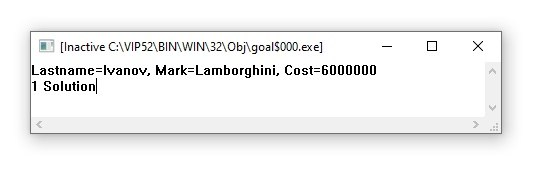
\includegraphics[scale=0.9]{img/1.jpg}
    \caption{Фамилия и марки автомобилей со стоимостью владельца номера 654321}
\end{figure}

\begin{lstlisting}[caption=Второй тест]
findWithPhone("123456" ,Mark).
\end{lstlisting}

\begin{figure}[H]
    \centering
    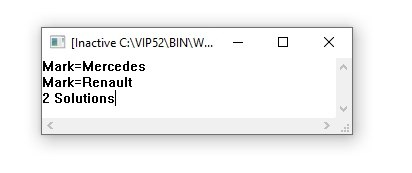
\includegraphics[scale=0.9]{img/2.jpg}
    \caption{Марки автомобилей владельца телефона 123456}
\end{figure}

\begin{lstlisting}[caption=Третий тест]
City = "Saint-Petersburg" ,
telephone("Ivanov", PhoneNumber, address(City, Street, _, _)),
deposit("Ivanov", Bank, _, _, City).
\end{lstlisting}

\begin{figure}[H]
    \centering
    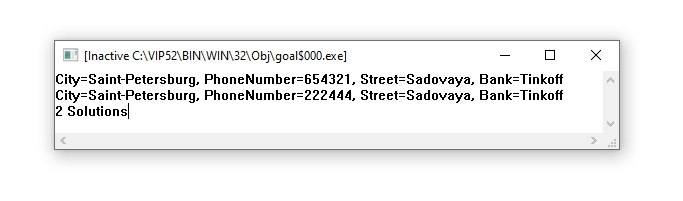
\includegraphics[scale=0.7]{img/3.jpg}
    \caption{Номер телефона, улица и банки, в которых вклады у Иванова из Санкт-Петербурга}
\end{figure}

\section{ПОРЯДОК ПОИСКА ОТВЕТА}

{
\small
\begin{longtable}{|p{1.15cm}|p{8cm}|p{8cm}|}
    \caption{findWithPhone(``654321'', Lastname, Mark, Cost).} \\
    \hline
    № шага & Сравниваемые термы: результат; подстановка, если есть & Дальнейшие действия: прямой ход или откат \\
    \hline
    1 & Подстановка: Number = ``654321''\ , Lastname = Lastname, Mark = Mark, Cost = Cost & Прямой ход \\
      & findWithPhone(``654321''\ , Lastname, Mark, Cost). & \\
      & findWithPhone(Number, Lastname, Mark, Cost). & \\
    \hline
    2 & Сравнение:  ``654321'' и ``123456'' & Прямой ход \\
      & telephone(\_, ``654321'', \_) & \\
      & telephone(``Ivanov'', ``123456'' , address(...)) & \\
    \hline
    3 & Сравнение: ``654321'' и ``654321'' & Прямой ход \\
      & telephone(\_, ``654321'', \_) & \\
      & telephone("Ivanov"\ , ``654321'', address(...)) & \\
    \hline
    4 & Подстановка: Lastname = ``Ivanov'', City = ``SP'' & Прямой ход \\
    \hline
    5 & Сравнение: ``Ivanov'' и ``Ivanov'', ``SP'' и ``Moscow'' & Прямой ход \\
      & car(Lastname, \_, \_, \_, City) & \\
      & car(``Ivanov'', ``Mercedes'', ``Black'', 3000000, ``Moscow'') & \\
    \hline
    6 & Сравнение: ``Ivanov'' и ``Ivanov'', ``SP'' и ``Moscow'' & Прямой ход \\
      & car(Lastname, \_, \_, \_, City) & \\
      & car(``Ivanov'', ``Renault'', ``Gray'', 1200000, ``Moscow'') & \\
    \hline
    7 & Сравнение: ``Ivanov'' и ``Ivanov'', ``SP'' и ``SP'' & Прямой ход \\
      & car(Lastname, \_, \_, \_, City) & \\
      & car(``Ivanov'', ``Lamborghini'', ``Yellow'', 6000000, ``SP'') & \\
    8 & Подстановка: Mark = ``Lamborghini'', Cost = 6000000 & Прямой ход \\
    \hline
    9 & \textbf{Результат} & Откат \\
      & \textbf{Lastname = ``Ivanov'', Mark = ``Lamborghini'', Cost = 6000000} & \\
    \hline
    10 & Сравнение: ``Ivanov'' и ``Petrov'', ``SP'' и ``Moscow'' & Прямой ход \\
      & car(Lastname, \_, \_, \_, City) & \\
      & car(``Petrov'', ``Audi'', ``Red'', 2000000, ``Moscow'') & \\
    \hline
    11 & Сравнение: ``Ivanov'' и ``Petrov'', ``SP'' и ``Moscow'' & Откат \\
      & car(Lastname, \_, \_, \_, City) & \\
      & car(``Petrov'', ``Infiniti'', ``Black'', 4000000, ``Moscow'') & \\
    \hline
    12 & Сравнение:  ``654321'' и ``222444'' & Прямой ход \\
      & telephone(\_, ``654321'', \_) & \\
      & telephone(``Ivanov'', ``222444'' , address(...)) & \\
    \hline
    13 & Сравнение:  ``654321'' и ``554322'' & Прямой ход \\
      & telephone(\_, ``654321'', \_) & \\
      & telephone(``Petrov'', ``554322'' , address(...)) & \\
    \hline
    14 & Сравнение:  ``654321'' и ``223544'' & Откат \\
      & telephone(\_, ``654321'', \_) & \\
      & telephone(``Petrov'', ``223544'' , address(...)) & \\
    \hline
\end{longtable}
}

{
\small
\begin{longtable}{|p{1.15cm}|p{8cm}|p{8cm}|}
    \caption{findWithPhone(``123456'', Mark)} \\
    \hline
    № шага & Сравниваемые термы: результат; подстановка, если есть & Дальнейшие действия: прямой ход или откат \\
    \hline
    1 & Подстановка: Number = "123456"\ , Mark = Mark & Прямой ход \\
        & findWithPhone("123456"\ , Mark) & \\
        & findWithPhone(Number, Mark) & \\
    \hline
    2 & Подстановка: Number = Number\ , Mark = Mark & Прямой ход \\
        & findWithPhone(Number, Mark) & \\
        & findWithPhone(Number, \_, Mark, \_) & \\
    \hline
    3 & Подстановка: Number = Number, Mark = Mark & Прямой ход \\
        & findWithPhone(Number, \_, Mark, \_) & \\
        & findWithPhone(Number, Lastname, Mark, Cost) & \\
    \hline
    4 & Сравнение: "123456" и "123456"& Прямой ход \\
        & telephone(Lastname, Number, address(City, \_, \_, \_)) & \\
        & telephone("Ivanov"\ , "123456"\ , address(...)) & \\
    \hline
    5 & Подстановка Lastname = "Ivanov"\ , City = "Moscow"& Прямой ход \\
        & telephone(Lastname, Number, address(City, \_, \_, \_)) & \\
        & telephone("Ivanov"\ , "123456"\ , address(...)) & \\
    \hline
    6 & Сравнение: "Ivanov" и "Ivanov", "Moscow" и "Moscow" & Прямой ход \\
        & car(Lastname, Mark, \_, \_, City) & \\
        & car("Ivanov"\ , "Mercedes"\ , "Black"\ ,3000000, "Moscow") & \\
    \hline
    7 & \textbf{Результат} & Откат \\
        & \textbf{Mark = "Mercedes"} & \\
    \hline
    8 & Сравнение: "Ivanov" и "Ivanov", "Moscow" и "Moscow" & Прямой ход \\
        & car(Lastname, Mark, \_, \_, City) & \\
        & car("Ivanov"\ , "Renault"\ , "Gray"\ ,1200000, "Moscow") & \\
    \hline
    9 & \textbf{Результат} & Откат \\
        & \textbf{Mark = "Renault"} & \\
    \hline
    10 & Сравнение: "Ivanov" и "Ivanov", "Moscow" и "SP" & Прямой ход \\
        & car(Lastname, Mark, \_, \_, City) & \\
        & car("Ivanov"\ , "Lamborghini"\ , "Yellow"\ ,6000000, "SP") & \\
    \hline
    11 & Сравнение: "Ivanov" и "Petrov", "Moscow" и "Moscow" & Прямой ход \\
        & car(Lastname, Mark, \_, \_, City) & \\
        & car("Petrov"\ , "Audi"\ , "Red"\ ,2000000, "Moscow") & \\
    \hline
    12 & Сравнение: "Ivanov" и "Petrov", "Moscow" и "Moscow" & Откат \\
        & car(Lastname, Mark, \_, \_, City) & \\
        & car("Petrov"\ , "Infiniti"\ , "Black"\ ,4000000, "Moscow") & \\
    \hline
    13 & Сравнение: "123456" и "654321"& Прямой ход \\
        & telephone(Lastname, Number, address(City, \_, \_, \_)) & \\
        & telephone("Ivanov"\ , "654321"\ , address(...)) & \\
    \hline
    14 & Сравнение: "123456" и "222444"& Прямой ход \\
        & telephone(Lastname, Number, address(City, \_, \_, \_)) & \\
        & telephone("Ivanov"\ , "222444"\ , address(...)) & \\
    \hline
    15 & Сравнение: "123456" и "554322"& Прямой ход \\
        & telephone(Lastname, Number, address(City, \_, \_, \_)) & \\
        & telephone("Petrov"\ , "554322"\ , address(...)) & \\
    \hline
    16 & Сравнение: "123456" и "223544"& Откат \\
        & telephone(Lastname, Number, address(City, \_, \_, \_)) & \\
        & telephone("Petrov"\ , "223544"\ , address(...)) & \\
    \hline
\end{longtable}
}

{
\small
\begin{longtable}{|p{1.15cm}|p{8cm}|p{8cm}|}
    \caption{
        Lastname = ``Ivanov'', \\
        City = ``Saint-Petersburg'',\\
        telephone(Lastname, PhoneNumber, address(City, Street, \_, \_)),\\
        deposit(Lastname, Bank, \_, \_, City).
    } \\
    \hline
    № шага & Сравниваемые термы: результат; подстановка, если есть & Дальнейшие действия: прямой ход или откат \\
    \hline
    1 & Подстановка: Lastname = ``Ivanov'' & Прямой ход \\
    \hline
    2 & Подстановка: City = ``SP'' & Прямой ход \\
    \hline
    3 & Сравнение: ``Ivanov'' и ``Ivanov'', ``SP'' и ``Moscow'' & Прямой ход \\
      & telephone(Lastname , \_ , address(City, \_, \_, \_)) & \\
      & telephone(``Petrov'', ``123456'', address(``Moscow'', ``Pyshkinskaya'', 12, 13)) & \\
    \hline
    4 & Сравнение: ``Ivanov'' и ``Ivanov'', ``SP'' и ``SP'' & Прямой ход \\
      & telephone(Lastname , \_ , address(City, \_, \_, \_)) & \\
      & telephone(``Ivanov'', ``654321'', address(``SP'', ``Sadovaya'', 10, 127)) & \\
    \hline
    5 & Подстановка: PhoneNumber = ``654321'', Street = ``Sadovaya'' & Прямой ход \\
    \hline
    6 & Сравнение: ``Ivanov'' и ``Ivanov'', ``SP'' и ``Moscow'' & Прямой ход \\
      & deposit(Lastname, \_, \_, \_, City) & \\
      & deposit(``Ivanov'', ``Tinkoff'', ``111222333444'', 40000, ``Moscow'') & \\
    \hline
    7 & Сравнение: ``Ivanov'' и ``Ivanov'', ``SP'' и ``Moscow'' & Прямой ход \\
      & deposit(Lastname, \_, \_, \_, City) & \\
      & deposit(``Ivanov'', ``Sberbank'', ``444333222111'', 100000, ``Moscow'') & \\
    \hline
    8 & Сравнение: ``Ivanov'' и ``Ivanov'', ``SP'' и ``SP'' & Прямой ход \\
      & deposit(Lastname, \_, \_, \_, City) & \\
      & deposit(``Ivanov'', ``Tinkoff'', ``123456789000'', 150000, ``SP'') & \\
    \hline
    9 & \textbf{Результат} & Откат \\
      & \textbf{PhoneNumber = ``654321'', City = ``SP'', Street = ``Sadovaya'', Bank = ``Tinkoff''} & \\
    \hline
    10 & Сравнение: ``Ivanov'' и ``Petrov'', ``SP'' и ``Moscow'' & Прямой ход \\
      & deposit(Lastname, \_, \_, \_, City) & \\
      & deposit(``Petrov'', ``Alpha-bank'', ``222333111444'', 100000, ``Moscow'') & \\
    \hline
    11 & Сравнение: ``Ivanov'' и ``Petrov'', ``SP'' и ``Moscow'' & Откат \\
      & deposit(Lastname, \_, \_, \_, City) & \\
      & deposit(``Petrov'', ``Sberbank'', ``123123321321'', 120000, ``Moscow'') & \\
    \hline
    12 & Сравнение: ``Ivanov'' и ``Ivanov'', ``SP'' и ``SP'' & Прямой ход \\
      & telephone(Lastname , \_ , address(City, \_, \_, \_)) & \\
      & telephone(``Ivanov'', ``222444'', address(``SP'', ``Sadovaya'', 10, 127)) & \\
    \hline
    13 & Подстановка: PhoneNumber = ``222444'', Street = ``Sadovaya'' & Прямой ход \\
    \hline
    14 & Сравнение: ``Ivanov'' и ``Ivanov'', ``SP'' и ``Moscow'' & Прямой ход \\
      & deposit(Lastname, \_, \_, \_, City) & \\
      & deposit(``Ivanov'', ``Tinkoff'', ``111222333444'', 40000, ``Moscow'') & \\
    \hline
    15 & Сравнение: ``Ivanov'' и ``Ivanov'', ``SP'' и ``Moscow'' & Прямой ход \\
      & deposit(Lastname, \_, \_, \_, City) & \\
      & deposit(``Ivanov'', ``Sberbank'', ``444333222111'', 100000, ``Moscow'') & \\
    \hline
    16 & Сравнение: ``Ivanov'' и ``Ivanov'', ``SP'' и ``SP'' & Прямой ход \\
      & deposit(Lastname, \_, \_, \_, City) & \\
      & deposit(``Ivanov'', ``Tinkoff'', ``123456789000'', 150000, ``SP'') & \\
    \hline
    17 & \textbf{Результат} & Откат \\
      & \textbf{PhoneNumber = ``222444'', City = ``SP'', Street = ``Sadovaya'', Bank = ``Tinkoff''} & \\
    \hline
    18 & Сравнение: ``Ivanov'' и ``Petrov'', ``SP'' и ``Moscow'' & Прямой ход \\
      & deposit(Lastname, \_, \_, \_, City) & \\
      & deposit(``Petrov'', ``Alpha-bank'', ``222333111444'', 100000, ``Moscow'') & \\
    \hline
    19 & Сравнение: ``Ivanov'' и ``Petrov'', ``SP'' и ``Moscow'' & Откат \\
      & deposit(Lastname, \_, \_, \_, City) & \\
      & deposit(``Petrov'', ``Sberbank'', ``123123321321'', 120000, ``Moscow'') & \\
    \hline
    20 & Сравнение: ``Ivanov'' и ``Petrov'', ``SP'' и ``Moscow'' & Прямой ход \\
      & telephone(Lastname , \_ , address(City, \_, \_, \_)) & \\
      & telephone(``Petrov'', ``554322'', address(``Moscow'', ``Baumanskaya'', 7, 53)) & \\
    \hline
    21 & Сравнение: ``Ivanov'' и ``Petrov'', ``SP'' и ``Moscow'' & Откат \\
      & telephone(Lastname , \_ , address(City, \_, \_, \_)) & \\
      & telephone(``Petrov'', ``223544'', address(``Moscow'', ``Baumankaya'', 7, 53)) & \\
    \hline
\end{longtable}
}

\section{ВОПРОСЫ}

\begin{enumerate}
    \item \textbf{Что такое терм?}
        \begin{enumerate}
            \item Константа
                \begin{itemize}
                    \item Число (целое, вещественное)
                    \item Символьный атом (комбинация символов латинского алфавита , цифр и нижнего подчеркивания, начинается со строчной буквы, используется для обозначения объекта или отношения)
                    \item Строка (последовательность символов, заключенная в кавычках)
                \end{itemize}

            \item Переменная
                \begin{itemize}
                    \item Именованная (комбинация символов латинского алфавита , цифр и нижнего подчеркивания, начинается с прописной буквы или символа подчеркивания)
                    \item Неименованная (обозначается символом подчеркивания)
                \end{itemize}
            \item Составной терм (имеет вид {\ttfamily f(t1, t2, ..., tm)})
        \end{enumerate}

    \item \textbf{Что такое предикат в матлогике(математике)?}

        Это функция с множеством значений $\{0;1\}$ (\{ложь;истина\}), определенное на множетсве $M=M_1 \times M_2 \times ... \times M_n$ так, что каждый набор $M$ определен как истинный или ложный.

    \item \textbf{Что описывает предикат в Prolog?}

        Предикат описывает какое-либо отношение.

    \item \textbf{Назовите виды предложений в програме и приведите примеры таких предложений из Вашей программы. Какие предложения являются основными, а какие -- не основными? Каковы: синтаксис и семантика (формальный смысл) этих предложений (основных и неосновных)?}

        \begin{itemize}
            \item \textbf{Факты} -- знания о том, что между аргументами существует отношение
                \begin{equation*}
                    f(t_1, t_2, ..., t_n)
                \end{equation*}

\begin{lstlisting}[caption=Пример факта (Основное предложение)]
telephone("Ivanov", "123456",
          address("Moscow", "Pyshkinskaya", 12, 13)
).
\end{lstlisting}

                Смысл -- человек с фамилией Ivanov и номером 123456 проживает по адресу: город Moscow, улица Pyshkinskaya, дом 12, квартира 13.

            \item \textbf{Правила}
                \begin{equation*}
                    A :- B_1, ..., B_n.
                \end{equation*}

                $A$ -- заголовок правила, $B_1, ..., B_n$ -- тело правила

\begin{lstlisting}[caption=Пример правила (Неосновное предложение)]
findWithPhone(Number, Lastname, Mark, Cost) :-
    telephone(Lastname, Number, address(City, _, _, _)),
    car(Lastname, Mark, _, Cost, City).
\end{lstlisting}

                Смысл -- Найти по номеру телефона фамилию, марку автомобиля и стоимость автомобиля с помощью отношения телефонной книги и владения автомобилем.

            \item \textbf{Вопросы}
                \begin{equation*}
                    f(X_1, X_2, ..., X_n)
                \end{equation*}

\begin{lstlisting}[caption=Пример вопроса (Несновное предложение)]
findWithPhone("123456", Mark).
\end{lstlisting}

            Смысл -- найти марку автомобилей, которае пренадлежат человеку, с номером 123456.
        \end{itemize}
    \item \textbf{Каковы назначение, виды и осоенности использования переменных в программе на Prolog? Какое предложение БЗ сформулирровано в более общей -- абстрактной форме: содержащее или не содержащее переменных?}

\begin{itemize}
    \item Именованная -- обозначается комбинацией символов латинского алфавита, цифр и символа подчеркивания, начинающейся с прописной буквы или символа подчеркивания (X, Student, \_X)
    \item Анонимная -- обозначается символом почеркивания (\_)
\end{itemize}

Переменные в момент фиксации утверждений в программе, обозначая некоторый неизвестный объект из некоторого множества объектов, не имеют значения. Значения для переменных могут быть установлены Prolog-системой только в процессе поиска ответа на вопрос, то есть реализации программы.

Переменные предназначены для передачи значений <<во времени и пространстве>>. Переменные в факты и правила входят только с квантором всеобщности. А в вопросы переменные входят только с квантором существования.

В процессе выполнения программы переменные могут сязываться с различными объектами -- \textbf{конкретизироваться}. Это относится только к именованным переменным. Анонимные переменные не могут быть связаны со значением.

В более общей -- абстрактной форме смормулировано предложение содержащее переменные.

    \item \textbf{Что такое подстановка?}

        Пусть дан терм $A(X_1, X_2, ..., X_n)$. \textbf{Подстановкой} называется множество пар, вида $\{X_i = t_i\}$, где $X_i$ -- переменная, а $t_i$ -- терм. Пусть $\Theta = \{ X_1 = t_1, X_2 = t_2, ..., X_n = t_n \}$ -- подстановка, тогда результат применения подстановки к терму обозначается $A\Theta$. Применение подстановки заключается в замене каждого вхождения переменной $X_i$ на соотвествующий терм.

    \item \textbf{Что такое пример терма? Как и когда строится? Как Вы думаете, система строит и хранит примеры?}

        Терм $B$ называется \textbf{примером} терма $A$, если существует такая подстановка $\Theta$, что $B = A\Theta$. Пример терма строится во время поиска решений при подстановке. Для построения примеров, система связывает переменные с конкретными термами, все примеры для текущего вопроса хранятся в стеке.
\end{enumerate}
